%!TEX root =presentation.tex
\subsection[complexity]{Complexity analysis of adjoint method} % (fold)
\label{sec:complexity_analysis_of_adjoint_method}

\begin{frame}[t]\frametitle{Complexity of solving gradient}
    




\begin{block}{Solving adjoint system}
\begin{equation}
    \Hx^T \lambda = -\Jx^T
\end{equation}
From previous result, $\Hx$ has following properties:

\begin{itemize}
    \item size $\ntime\nlinks \times \ntime\nlinks$
    \item lower triangular
    \item $card\,\Hx = O(\nlinks\ntime\degree{\state})$: $\degree{\state}=\max_{\jn\in\jns}\left(\ninc_{\jn}+\nout_{\jn}\right)$
\end{itemize}

Efficiently solve $\lambda$ via backward-substitution in time $O(\ntime \nlinks \degree{\state})$, or \textbf{linear in $\ntime \nlinks$}.
\end{block}
\end{frame}

\begin{frame}[t]\frametitle{Complexity of solving gradient}

\begin{block}{Solving $\nabla \cost$}
\begin{equation}
    \nabla \cost = \lambda^T \Hu + \Ju
\end{equation}

From previous result, $\Hu$ has following properties:

\begin{itemize}
    \item size $\ntime\nlinks \times  \ntime \ncontrols$
    \item $card\,\Hu = O(\ntime \nlinks \degree{\control})$: $\degree{\control}=\max_{\condiscrete{}{}\in\control}\sum_{\jn\in\jns:\condiscrete{}{}\in\junccon{\jn}{\tind}}\left(\ninc_{\jn}+\nout_{\jn}\right)$
\end{itemize}

Sparse matrix multiplication has total cost $O(\ntime \ncontrols \degree{\control})$.
\end{block}

\end{frame}

\begin{frame}
\begin{figure}
\begin{centering}
\subfloat[\label{fig:genneta}]{\begin{centering}
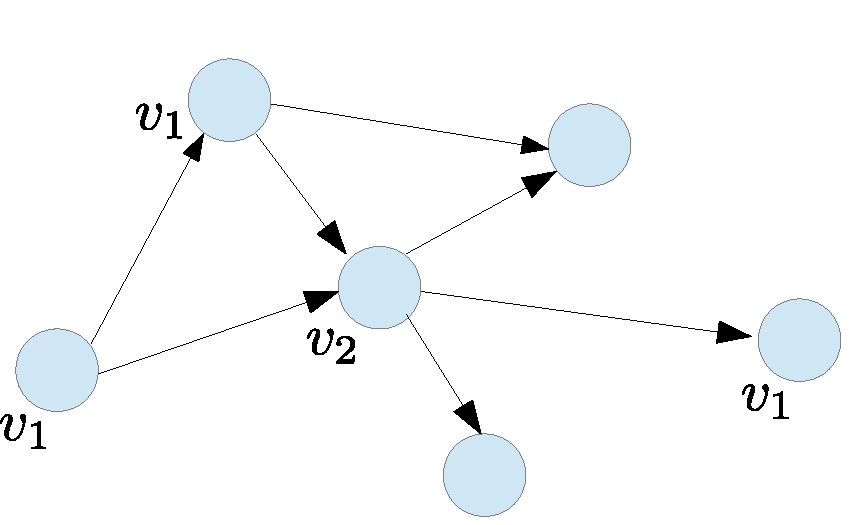
\includegraphics[width=0.33\columnwidth]{../figs-gen/gen-net}
\par\end{centering}

}\subfloat[\label{fig:gennetb}]{\begin{centering}
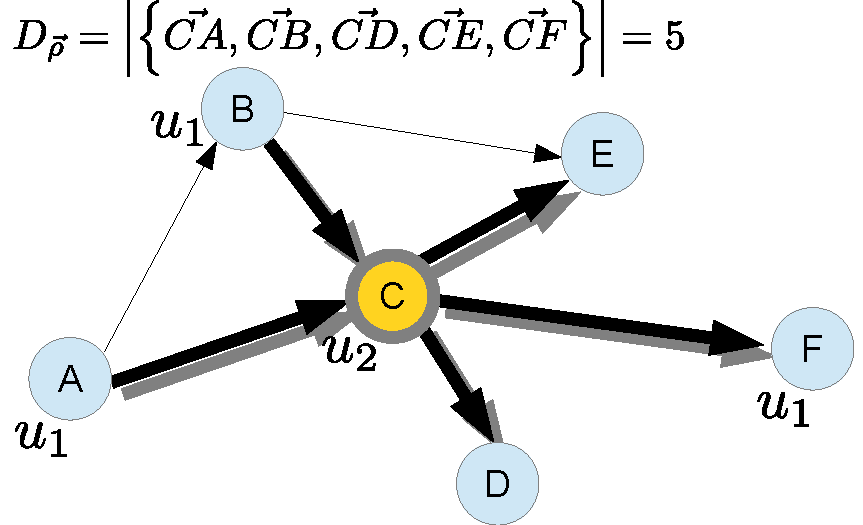
\includegraphics[width=0.33\columnwidth]{../figs-gen/gen-net-dx}
\par\end{centering}

}\subfloat[\label{fig:gennetc}]{\begin{centering}
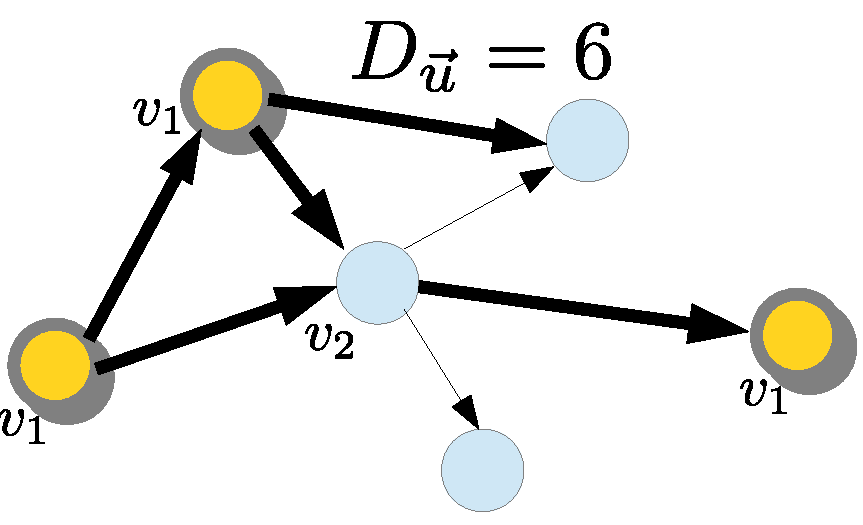
\includegraphics[width=0.33\columnwidth]{../figs-gen/gen-net-dv}
\par\end{centering}

}
\par\end{centering}
\end{figure}
\end{frame}


\begin{frame}[t]\frametitle{Complexity of solving gradient}
    
\begin{block}{Total complexity of computing gradient via discrete adjoint}
\[
O(\ntime\left(\degree{\state}\nlinks+\degree{\control}\ncontrols\right))
\]
\end{block}

\begin{figure}
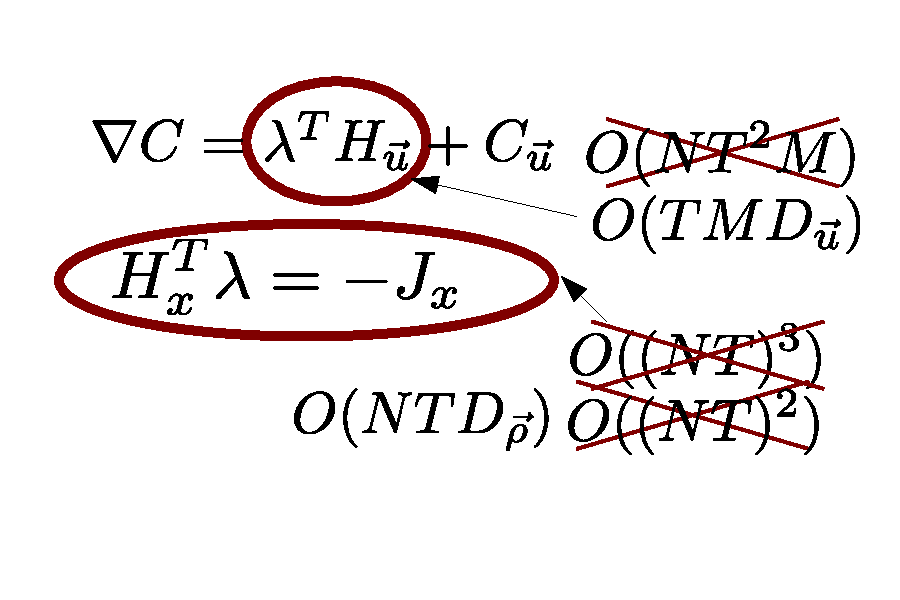
\includegraphics[width=.8\columnwidth]{figs-gen/complexity}
\end{figure}
\end{frame}



% section complexity_analysis_of_adjoint_method (end)